\documentclass[notes,color]{sepslide0}
\usepackage{graphicx}
\usepackage[overheads]{mysepslides}
\usepackage{tech,graphicx,url,csp-cm,tikz,scalalistings}

\title{Monitors} 
\author{Gavin Lowe}

% \everymath{\color{Plum}}
\def\smaller{\small} 
\def\scalacolour{\color{violet}}

\begin{document}

\begin{slide}
  
  \Title

Reading: Andrews Chapter 5.
\end{slide}

%%%%%


\begin{slide}
\heading{Low-level concurrency mechanisms}

So far, we have looked at threads that communicate via channels.

At a higher level of abstraction, we have looked at threads that communicate
via concurrent datatypes. 

We now look at the low-level concurrency primitives provided by the language.
(These can be used to implement high-level concurrency mechanisms such as
channels; or can be used to implement concurrent datatypes.) 
\end{slide}

%%%%%

\begin{slide}
\heading{A race condition}

The following program has an obvious race condition.
%
\begin{scala}
object Race2{
  object Counter{
    private var x = 0
    def inc = x = x+1
    def dec = x = x-1
    def getX = x
  }

  def p = thread{ for(i <- 0 until 1000) Counter.inc }
  def q = thread{ for(i <- 0 until 1000) Counter.dec }
  def system = p || q

  def main(args : Array[String]) = { run(system); println(Counter.getX) }
}
\end{scala}
\end{slide}

%%%%%

\begin{slide}
\heading{Mutual exclusion}

The program on the previous slide allowed the two processes \SCALA{p} and
\SCALA{q} to simultaneously access the variable \SCALA{Counter.x}, via the
\SCALA{inc} and \SCALA{dec} operations.

We would like to ensure that the operations \SCALA{inc} and \SCALA{dec} are
performed under \emph{mutual exclusion}: i.e.~at most one of them can be
performed at a time.  
\end{slide}

%%%%%

\begin{slide}
\heading{Monitors}

An \emph{object} encapsulates data and operations on that data.

A \emph{monitor} encapsulates data, operations on that data, and suitable
synchronisations to ensure mutual exclusion.

In order to execute code in the monitor, a thread must first of all obtain the
lock on the monitor.  The thread releases the lock when it exits the monitor.
\end{slide}

%%%%%

\begin{slide}
\heading{Signalling}

In addition, a monitor sometimes requires a thread to wait until it receives a
signal from another thread.  

For example, consider a partial queue.  If a thread attempting to dequeue
finds that the queue is empty, it should wait.  When an enqueue operation
makes the queue non-empty, it can signal to the waiting thread.
\end{slide}

%%%%%

\begin{slide}
\heading{Monitors}

The way to ensure mutual exclusion within a Scala object  is via the
\SCALA{synchronized} method.  

If |o| is a reference object and \SCALA{e} is an expression, then
\SCALA{o.synchronized\{ e \}} acts much like \SCALA{e}, except that at most
one thread can be active within the \SCALA{synchronized} expressions of the
monitor~|o| at any time.  Note that |o| must be a reference object (a subclass
of |AnyRef|), not, for example, an |Int|. 

If a thread tries to execute a \SCALA{synchronized}
expression while another thread is active within the monitor, then the former
thread has to wait until the latter releases the lock. 

This can be used to ensure that executions of code within
|synchronized| blocks do not interfere with one another. 

|synchronized{ e }| is shorthand for |this.synchronized{ e }|; i.e.~the
current object is used for the synchronisation.
\end{slide}

%%%%%

\begin{slide}
\heading{Using \protect\SCALA{synchronized} to avoid a race condition}

\begin{scala}
object Race3{
  object Counter{
    private var x = 0
    def inc = synchronized{ x = x+1 }
    def dec = synchronized{ x = x-1 }
    def getX = synchronized{ x }
  }

  def p = thread{ for(i <- 0 until 1000) Counter.inc }
  def q = thread{ for(i <- 0 until 1000) Counter.dec }
  def system = p || q

  def main(args : Array[String]) = { run(system); println(Counter.getX) }
}
\end{scala}
\end{slide}

%%%%%

\begin{slide}
\heading{Example: a concurrent set}

Here's an implementation of the concurrent set we used in the
breadth-first search example. 
\begin{scala}
/** A concurrent set with an add operation. */
class ConcSet[A]{
  /** The underlying set. */
  private val set = scala.collection.mutable.Set[A]()

  /** Add x to this set.  Return true if x was not previously in the set. */
  def add(x: A): Boolean = synchronized{ set.add(x) }
}
\end{scala}

Additional operations can be added similarly. 
\end{slide}

%%%%%

\begin{slide}
\heading{Re-entry}

A thread inside a |synchronized| block can enter another |synchronized| block
on the same object.  For example
%
\begin{scala}
  synchronized{
    ...
    synchronized{ ... }
    ...
  }
\end{scala}
%
Or
%
\begin{scala}
def f(x: Int) = synchronized{ ...; g(y); ... }
def g(y: Int) = synchronized{ ... }
\end{scala}

We say that |synchronized| blocks are \emph{re-entrant}. 
\end{slide}
 % intro, race condition examples.


\begin{slide}
\heading{A producer-consumer problem}

Consider the following producer-consumer problem (with a single producer and
single consumer).  The producer produces some data which it puts into a
``slot''.  The consumer gets the data and operates on it.  The consumer should
process each piece of data precisely once.  We want |put| and |get| operations
to support this. 

The consumer needs to be able to identify whether the data currently
in the slot is new or not, for which we use a boolean flag \SCALA{filled}.
%
\begin{itemize}
\item The producer waits until \SCALA{filled = false} before filling the slot,
and then sets \SCALA{filled} to \SCALA{true}.

\item The consumer waits until \SCALA{filled = true} before taking the data,
and then sets \SCALA{filled} to \SCALA{false}.
\end{itemize}

% (Alternatively, we could use an |Option| value, with |None| representing that
% the slot is empty.)
\end{slide}

%%%%%

\begin{slide}
\heading{Busy waiting}

Here's a definition that looks like it should work, but doesn't.

\begin{scala}
class Slot[T]{
  private var value = null.asInstanceOf[T] // current or previous item
  private var filled = false                 // if value valid?

  def put(v: T) = {
    while(filled){  } // spin
    value = v; filled = true
  }

  def get : T = {
    while(!filled){  } // spin
    val result = value; filled = false
    result
  }
}
\end{scala}
\end{slide}

%%%%%

\begin{slide}
\heading{Busy waiting}

The previous solution doesn't work because of compiler optimizations.  It
deadlocks after a few iterations.  I think  
\begin{scala}
    while(filled){  } 
\end{scala}
is ``optimized'' to something equivalent to
\begin{scala}
    if(filled){ while(true){} }
\end{scala}
by the JIT compiler.

Also, the compiler could reverse the order of the two assignments by |put|, or
could reverse the order of the two reads by |get|.  

Or the consumer could read a stale value of |value|, because of the use of
caches.
\end{slide}

%%%%%

\begin{slide}
\heading{Busy waiting}

Even if the code did work, it wouldn't be ideal.
%
% \begin{itemize}
% \item
The busy-waiting loop means both threads are using computational resources
unnecesarily.  This mechanism won't scale well, since if there are many
threads, they will be competing for access to the (limited) processors, and
also competing for use of the memory bus.

\emph{Do not use busy waiting.}

% \item
% Both processes need access to the object simultaneously, so we can't turn it
% into a monitor.  This doesn't matter in this case, but it would in others.

%% \item
%% The Java memory model makes no guarantee that the value of \SCALA{value} is
%% copied from the processor's cache to main memory.

%% \item
%% The compiler is allowed to perform optimisations to reverse the order of the
%% writes to \SCALA{value} and \SCALA{empty}.
%\end{itemize}

What we would like to do is arrange for the producer thread to wait (suspend)
until notified by the consumer thread that it can proceed.  Similarly, we
would like the consumer thread to wait (suspend) until notified by the
producer thread that it can proceed.
\end{slide}

%%%%%

\begin{slide}
\heading{Using {\scalashape wait} and {\scalashape notify}}

\begin{scala}
class Slot[T]{
  private var value = null.asInstanceOf[T] // current or previous item
  private var filled = false                 // if value valid?

  def put(v: T) = synchronized{
    while(filled) wait() // wait for the slot to be emptied
    value = v; filled = true
    notify()  // notify the consumer
  }

  def get : T = synchronized{
    while(!filled) wait() // wait for the slot to be filled
    val result = value; filled = false
    notify()  // notify the producer
    result
  }
}
\end{scala}
\end{slide}

%%%%%

\begin{slide}
\heading{{\scalashape wait} and {\scalashape notify}}

When a thread executes \SCALA{wait()}, it is suspended and gives up
the lock.  If waits until another thread
in the same monitor executes \SCALA{notify()}, at which point it becomes
\emph{ready} to run.  

However, it cannot run until it obtains the lock on the monitor: the thread
that performed the \SCALA{notify()} must release the lock; and the awakened
thread has to compete with other threads to obtain the lock.

Also, the implementation of |wait| is buggy.  Sometimes a thread doing a
|wait()| will wake up even though there was no |notify()|: a \emph{spurious
  wake-up}.
\end{slide}

%%%%%

\begin{slide}
\heading{Thread states}

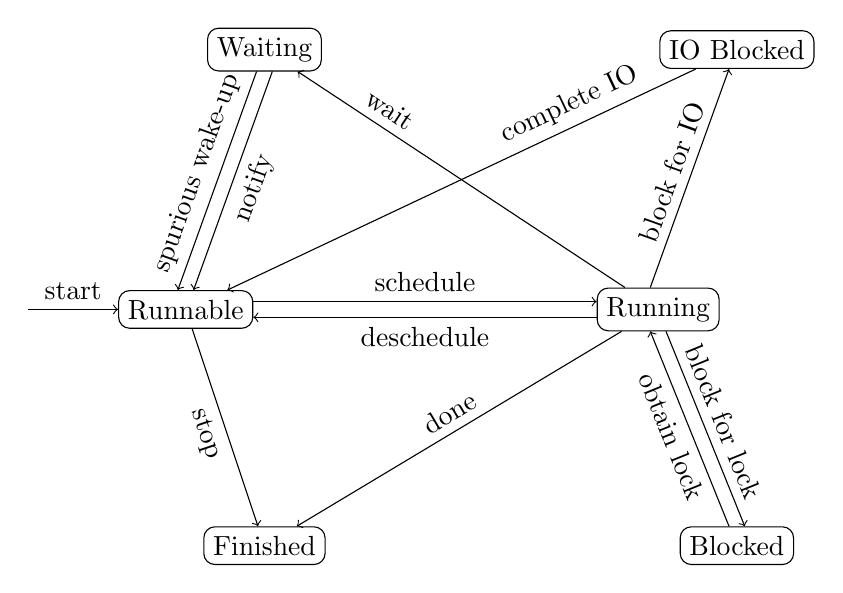
\begin{tikzpicture}
\draw(0,0) node[draw, rounded corners](runnable){Runnable};
\draw[<-] (runnable) -- node[above]{start} (-2,0);
%
\draw(6,0) node[draw, rounded corners](running){Running};
\draw[->] ([yshift = 1mm] runnable.east) -- node[above]{schedule} 
  ([yshift = 1mm] running.west);
\draw[->] ([yshift = -1mm] running.west) -- node[below]{deschedule} 
  ([yshift = -1mm] runnable.east);
% Waiting
\draw (1,3.3) node[draw, rounded corners](waiting){Waiting};
\draw[->] (running) -- node[above, sloped, near end]{\scalashape wait} (waiting);
\draw[->] ([xshift = -1mm] waiting.south) -- node[above, sloped]
  {spurious wake-up} ([xshift = -1mm] runnable.north);
\draw[->] ([xshift = 1mm] waiting.south) -- node[below, sloped]
  {\scalashape notify} ([xshift = 1mm] runnable.north);
%
\draw (1, -3) node[draw, rounded corners](finished){Finished};
\draw[->] (runnable) -- node[below, sloped]{stop} (finished);
\draw[->] (running) -- node[above, sloped]{done} (finished);
%
\draw(7, -3) node[draw, rounded corners](blocked){Blocked};
\draw[->] ([xshift = 1mm] running.south) -- 
  node[above, sloped]{block for lock} ([xshift = 1mm] blocked.north);
\draw[->] ([xshift = -1mm] blocked.north) -- node[below, sloped]{obtain lock} 
  ([xshift = -1mm] running.south);
% IO Blocked
\draw(7, 3.3) node[draw, rounded corners](IOblocked){IO Blocked};
\draw[->] ([xshift = -1mm] running.north) -- 
  node[above, sloped]{block for IO} ([xshift = -1mm] IOblocked.south);
\draw[->] ([xshift = 1mm] IOblocked) -- 
  node[above, sloped, near start]{complete IO} 
  (runnable);
\end{tikzpicture}

% \begin{center}
% \includegraphics[width=12cm]{Pics/threadStates.eps}
% \end{center}
\end{slide}

%%%%%

\begin{slide}
\heading{{\scalashape wait} and {\scalashape notify}}

Normally, a thread performs a \SCALA{wait} because some condition~\SCALA{cond}
is false, and it needs to wait for~\SCALA{cond} to become true.  

Normal practice is for another thread to perform a |notify| only when the
condition becomes true.

However, because of the possibility of spurious wake-ups, the awoken thread
should re-check the  condition~\SCALA{cond}.  The correct form of waiting is
%
\begin{scala}
  while(!cond) wait()
\end{scala}

Further, even without the possibility of spurious wake-ups, some third thread
might have run before the awoken thread, and so made the condition false. 

% Further, sometimes a thread will wake up without being notified, due to bugs
% in the implementation of Java --- a so-called \emph{spurious wakeup}.  These
% occur rarely in practice, but you should still guard against them, for example
% by using the above form of waiting.
\end{slide}

%%%%%

\begin{slide}
\heading{{\scalashape wait} and {\scalashape notify}}

When a thread performs |wait| or |notify|, it must be inside a corresponding
|synchronized| block on the same object, either the current object (|this|):
\begin{scala}
synchronized{ ... wait() ... notify() ... }
\end{scala}
%
or some other reference object~|o|:
\begin{scala}
o.synchronized{ ... o.wait() ... o.notify() ... }
\end{scala}
\end{slide}

%%%%%

\begin{slide}
\heading{Multiple producers and consumers}

Suppose we run the |Slot| with multiple producers and consumers.  It turns out
that previous implementation works incorrectly.
%
Consider the following execution, if |notify| is used.
%
\begin{enumerate}
\item Two consumers run, and both have to wait.

\item Producer~1 runs, sets |filled = true|, wakes up consumer~1, and returns.

\item Producer~2 runs, but has to wait.

\item Consumer~1 runs, sets |filled = false|, calls |notify()| which wakes up
consumer~2, and returns.

\item Consumer~2 runs, finds |filled = false|, so waits again. 
\end{enumerate}
%
Now producer~2 and consumer~2 are both waiting, but they should have been able
to exchange data. 

% If consumer~1 calls |notifyAll|, things will work correctly. 
\end{slide}

%%%%%

\begin{slide}
\heading{\scalashape notifyAll}


\SCALA{notify()} wakes up just one thread (if there is one waiting).  By
contrast, \SCALA{notifyAll()} wakes up \emph{all} threads waiting in this
monitor. 

Note that \SCALA{notifyAll()} is an expensive operation: all the waiting
threads will be awoken, obtain the lock, check the guard on their wait loop,
and normally all but one will immediately do another \SCALA{wait}.
\end{slide}

%%%%%

\begin{slide}
\heading{A slot for multiple producers and consumers}

\begin{scala}
class Slot2[T]{
  private var value = null.asInstanceOf[T]
  private var filled = false

  def put(v:T) = synchronized{
    while(filled) wait()
    value = v; filled = true; notifyAll()
  }

  def get : T = synchronized{
    while(!filled) wait()
    filled = false; val result = value; notifyAll(); result
  }
}
\end{scala}
%
\end{slide}

%%%%%

\begin{slide}
\heading{A slot for multiple producers and consumers}

Note that in this case it would be necessary for an awoken thread to recheck
the condition even if spurious wake-ups didn't exist: it is possible that some
other thread has run and invalidated the condition in the meantime.

Having to use |notifyAll| is inefficient.  It would be better if |get| could
target a |notify| towards a |put|, and vice versa.  We'll see a way to achieve
this effect in a later chapter.
\end{slide}

%%%%%

\begin{slide}
\heading{Signal-and-continue versus signal-and-wait}

Note that Scala (like Java) uses \emph{signal-and-continue} semantics: when a
thread signals, it continues to hold the lock on the monitor; the
awakened thread must wait to get the lock.  That means that we could have
written |get| as 
%
\begin{scala}
  def get : T = synchronized{
    while(!filled) wait() // wait for the slot to be filled
    filled = false
    notify() // notify the producer
    value
  }
\end{scala}

By contrasts, some systems use \emph{signal-and-wait} semantics, where the
thread that signals also gives up the lock; the awakened thread runs.
\end{slide}

%%%%%

% \begin{slide}
% \heading{Exercise}

% Adapt the |Slot| example to hold an (unbounded) partial queue of data.
% \end{slide}


%%%%%

% \begin{slide}
% \heading{Caches and memory optimisations}

% The original version of the slot has some additional subtle problems:
% %
% \begin{itemize}
% \item
% The Java memory model makes no guarantee that the value of \SCALA{value} is
% copied from the processor's cache to main memory.

% \item
% The compiler is allowed to perform optimisations to reverse the order of the
% writes to \SCALA{value} and \SCALA{empty}.
% \end{itemize}
% \end{slide}

%%%%%

\begin{slide}
\heading{Java Memory Model}

Recall that the original version of the slot has some subtle problems caused
by the Java Memory Model.  The use of |wait| and |notify| avoids these.

When a thread exits a |synchronized| block (either at the end of a
procedure, or by performing a \SCALA{wait}), it \emph{publishes} the
values in the cache, making them available to other threads.

When a thread enters a |synchronized| block (either initially, or after
receiving a \SCALA{notify}), it \emph{subscribes} to all variables
published by other threads on the same monitor.

Compiler optimisations must respect this semantics.

This means that if you are using |synchronized| blocks correctly to protect
against data races, you do not need to worry about the Java Memory Model. 


%% \footnote{\url{http://www.cs.umd.edu/~pugh/java/memoryModel/jsr-133-faq.html}}
%\vfill
\end{slide}


%%%%%

\begin{slide}
\heading{{\scalashape wait(t)}}

\SCALA{wait(t)} acts like \SCALA{wait()}, except it will wake up after
\SCALA{t}ms, if it hasn't been woken by a \SCALA{notify} in the meantime.
This can be used to implement timeouts.  

%% \SCALA{notify()} wakes up just one thread (if there is one waiting).  By
%% contrast, \SCALA{notifyAll()} wakes up \emph{all} threads waiting in this
%% monitor. 

%% See the API documentation for \SCALA{Scala.AnyRef} and
%% \SCALA{java.lang.Object} for more details.

%% Note that \SCALA{notifyAll()} is an expensive operation: all the waiting
%% threads will be awoken, obtain the lock, check the guard on their wait loop,
%% and normally all but one will immediately do another \SCALA{wait}.

%% All calls to each of |wait|, |notify| and |notifyAll| must be from inside a
%% |synchronized| block.
\end{slide}
 % producer-consumer example, with one of each
% \input{monitors3} % multiple producers and consumers; CSO conditions
\begin{slide}
\heading{A synchronous channel}

We will adapt the |Slot| example to implement a synchronous channel, suitable
for use by a \emph{single} sender and a \emph{single} receiver.

We need to arrange for the sender to wait until it receives a signal from
the receiver. 
\end{slide}

%%%%%

\begin{slide}
\heading{A synchronous channel}

\begin{scala}
/** A one-one synchronous channel passing data of type A, implemented using a
  * monitor. */
class SyncChan[A]{
  /** The current or previous value. */
  private var value = null.asInstanceOf[A]

  /** Is the current value of £value£ valid, i.e. ready to be received? */
  private var full = false

  /** Send x on the channel, synchronously. */
  def send(x: A) = ...

  /** Receive a value on the channel. */
  def receive: A = ...
}
\end{scala}
\end{slide}


%%%%%

\begin{slide}
\heading{A synchronous channel}

\begin{scala}
  def send(x: A) = synchronized{
    assert(!full)           // previous round must be complete
    value = x; full = true // deposit my value 
    notify()                // signal to receiver at (2)
    while(full) wait()      // wait for receiver (1)
  }

  def receive: A = synchronized{
    while(!full) wait()     // wait for sender (2)
    full = false            // clear value 
    notify()                // notify sender at (1)
    value
  }
\end{scala}
\end{slide}

%%%%%

\begin{slide}
\heading{Testing}

We can test the channel using logging.  We arrange for a single sender and a
single receiver to use the channel, writing events to the log before and after
each operation.  We then traverse the log, checking that no call returns
before both the |send| and |receive| operations have been called, and that
each value received matches the value sent. 
\end{slide}


\begin{slide}
\heading{Readers and writers}

The \emph{readers and writers problem} is a classic synchronisation problem.
Consider a collection of processes, each of which want to access a database
concurrently, some for reading and some for writing.  It is allowable for
several readers to be accessing the database simultaneously, since their
transactions will be independent.  However, it is not allowable for two
writers to have simultaneous access, nor for a reader and writer to have
simultaneous access.
\end{slide}

%%%%%


\begin{slide}
\heading{Readers and writers}

We will implement a controller object that controls access to the database,
implementing the following trait.
\begin{scala}
/** Trait for a readers and writers lock. */
trait ReadersWritersLock{
  def readerEnter: Unit
  def readerLeave: Unit
  def writerEnter: Unit
  def writerLeave: Unit
}
\end{scala}
%
The |Enter| methods will block, until the thread is allowed to use the
database. 
\end{slide}

%%%%%

\begin{slide}
\heading{Readers and writers}

The readers and writers call the appropriate operation before
and after  using the database; for example:
%
\begin{scala}
def reader(me: Int, rw: ReadersWritersLock) = thread{
  repeat{
    <operations not using database>
    rw.readerEnter // entry protocol
    <read the database>
    rw.readerLeave // exit protocol
  }
}
\end{scala}
\end{slide}

%%%%%

\begin{slide}
\heading{A simple implementation}

The |ReadersWritersLock| needs to keep track of the number of readers and
writers currently using the database, and maintain a suitable invariant.
%
\begin{scala}
class ReadersWritersMonitor extends ReadersWritersLock{
  private var readers = 0; private var writers = 0
  // Invariant: writers <= 1 && (readers == 0 || writers == 0)
  ...
}    
\end{scala}
\end{slide}

%%%%%

\begin{slide}
\heading{A simple implementation}

\begin{scala}
  def readerEnter = synchronized{
    while(writers > 0) wait()
    readers += 1
  }

  def readerLeave = synchronized{
    readers -= 1; notifyAll()
  }

  def writerEnter = synchronized{
    while(writers > 0 || readers > 0) wait()
    writers = 1
  }
      
  def writerLeave = synchronized{
    writers = 0; notifyAll()
  }
\end{scala}
\end{slide}


% \begin{slide}
% \heading{The controller}

% The controller needs to keep track of the number of readers and writers
% currently using the database, and maintain the following invariant:
% \begin{scala}
% readers==0 && writers<=1 || writers==0
% \end{scala}
% \end{slide}

% %%%%%

% \begin{slide}
% \heading{The controller}

% \begin{scala}
% object RWController{
%   private var readers = 0; private var writers = 0;
%   // Invariant readers==0 && writers<=1 || writers==0

%   def ReaderEnter = synchronized{
%     while(writers>0) wait();
%     readers+=1;
%   }

%   def WriterEnter = synchronized{
%     while(writers>0 || readers>0) wait();
%     writers=1;
%   }

%   ...
% }
% \end{scala}
% \end{slide}

% %%%%%

% \begin{slide}
% \heading{The controller}

% \begin{scala}
% object RWController{
%   ...

%   def ReaderLeave = synchronized{
%     readers-=1; notifyAll();
%   }
      
%   def WriterLeave = synchronized{
%     writers=0; notifyAll();
%   }
% }
% \end{scala}
% \end{slide}

%%%%%

\begin{slide}
\heading{Waking up}

Suppose a writer is currently accessing the database, and there are several
readers and writers waiting.  When the writer finishes and performs
|notifyAll|, all the waiting readers and writers become runnable.  One of
two things may occur:
%
\begin{itemize}
\item
A reader obtains the lock first, sets |readers = 1|, and accesses the database.
When the other writers are scheduled, they find \SCALA{readers > 0} and so
again \SCALA{wait}.  When the other readers are scheduled, they can also access
the database.

\item
A writer obtains the lock first, sets |writers = 1|, and accesses the
database.  When the other readers and writers are scheduled, they find
\SCALA{writers > 0} and so again \SCALA{wait}.
\end{itemize}
\end{slide}

%%%%%

\begin{slide}
\heading{Testing}

We can test the |ReadersWritersLock| by logging and then examining the log.
%
\begin{itemize}
\item Arrange for each thread to log entering and leaving the database
(for either reading or writing): logging entering should be done
\emph{after} entering, and logging leaving should be done
\emph{before} leaving:%
%
\begin{scala}
  rw.readerEnter; log.add(me, ReaderEnter)
  ...
  log.add(me, ReaderLeave); rw.readerLeave
\end{scala}
This ensures that the period between the log events is a subset of the period
when the thread is allowed to use the database, to avoid false positives.
      
\item When all threads have finished, traverse the log to ensure the invariant
was maintained.

\item Repeat many times.
\end{itemize}
%
%See the code on the website.
\end{slide}

%%%%%

\begin{slide}
\heading{Starvation}

The previous version of the readers-writers lock was unfair.  

Consider a scenario where readers repeatedly enter and leave the database, and
such that there is always at least one reader using it (even though no single
reader remains in the database).  The writers are starved!
\begin{center}
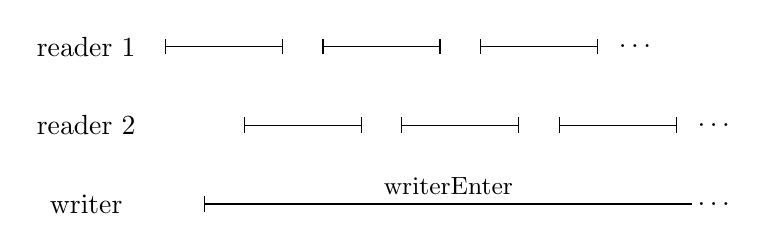
\begin{tikzpicture}
\draw (0,0) node{reader 1};
\draw[|-|] (1,0) -- (2.5,0); \draw[|-|] (3.0,0) -- (4.5,0); 
\draw[|-|] (5.0,0) -- (6.5,0); \draw (7.0,0) node{\ldots};
\draw (0,-1) node{reader 2}; 
\draw[|-|] (2.0,-1) -- (3.5,-1); \draw[|-|] (4.0,-1) -- (5.5,-1); 
\draw[|-|] (6.0,-1) -- (7.5,-1); \draw (8.0,-1) node{\ldots};
\draw (0,-2) node{writer}; 
\draw[|-] (1.5,-2) -- node[above]{\small\scalashape writerEnter} (7.7,-2);
\draw (8.0,-2) node{\ldots};
\end{tikzpicture}
\end{center}
\end{slide}

%%%%%

\begin{slide}
\heading{Avoiding starvation}

We give a fair version, using the following idea:
%
\begin{itemize}
\item Each writer registers its interest before actually entering the
database;

\item If a writer has registered its interest, no reader subsequently enters.
\end{itemize}
%
Thus eventually all the current readers will leave, and the writer can enter. 
\end{slide}

%%%%%

\begin{slide}
\heading{A fair readers-writers lock}

\begin{scala}
class FairReadWriteLock extends ReadersWritersLock{
  private var readers = 0 // current # readers in the CS
  private var writers = 0 // current # writers in the CS or trying

  def readerEnter = synchronized{
    while(writers > 0) wait() // wait for writer to leave
    readers += 1 // record my entry
  }

  def readerLeave = synchronized{
    readers -= 1 // record my exit
    if(readers == 0) notifyAll() // signal to waiting writer
  }
  ...
}
\end{scala}
\end{slide}

%%%%%

\begin{slide}
\heading{A fair readers-writers lock}

\begin{scala}
  def writerEnter = synchronized{
    while(writers > 0) wait() // wait until no writer ahead of me
    writers = 1 // record that I'm trying; readers are blocked
    while(readers > 0) wait() // wait for readers to leave
  }

  def writerLeave = synchronized{
    writers = 0 // record my exit
    notifyAll() // signal to waiting reader or writer
  }
\end{scala}

This avoids starvation provided the JVM monitor is fair.
\end{slide}

 % readers and writers lock

%%%%%%%%%%%%%%%%%%%%%%%%%%%%%%%%%%%%%%%%%%%%%%%%%%%%%%%%%%%%


%%%%%

% \begin{slide}
% \heading{Analysing synchronisation problems}

% We need better formal analysis techniques!
% \end{slide}

%%%%%

\begin{slide}
\heading{Summary}

\begin{itemize}
\item 
Enforcing mutual exclusion using \SCALA{synchronized}.

%% \item
%% Fine-grained locking; striped locking; sharding.

\item
\SCALA{wait}, \SCALA{notify}, \SCALA{notifyAll}.

\item
Thread states; signal-and-continue versus signal-and-wait.

\item
The Java memory model.

\item
Examples.
\end{itemize}

\end{slide}



\end{document}
